% Section for the appendix
\section{Appendix}\label{section:appendix}

% Subsection providing a link to the source code repository
\subsection{Source Code}
The interested reader can find the source code \href{https://github.com/HuberNicolas/gaia-classifier}{here}.

\section{Data}

\subsection{Feature Subsets}

% Table including symbolic notation
\begin{table}[h!]
    \centering
    \begin{tabular}{>{\raggedright\arraybackslash}m{3cm}>{\centering\arraybackslash}m{2cm}>{\centering\arraybackslash}m{2cm}>{\centering\arraybackslash}m{3cm}>{\centering\arraybackslash}m{2cm}}
    \hline
    \textbf{Dataset} & \textbf{Size} & \textbf{Accuracy} & \textbf{Symbol} & \textbf{Used} \\
    \hline
    Dataset A & 1000 & 92\% & $\dagger$ & \checkmark \\
    Dataset B & 5000 & 87\% & $x$ & \ding{55} \\
    Dataset C & 2000 & 95\% & $o$ & \checkmark \\
    \hline
    \multicolumn{5}{l}{$\dagger$: Symbol A, $x$: Symbol B, $o$: Symbol C} \\
    \end{tabular}
    \caption{Summary of Datasets and Accuracy}
    \label{tab:datasets}
\end{table}

\section{Evaluation}

% Figure
\begin{figure}[H]
    \centering
    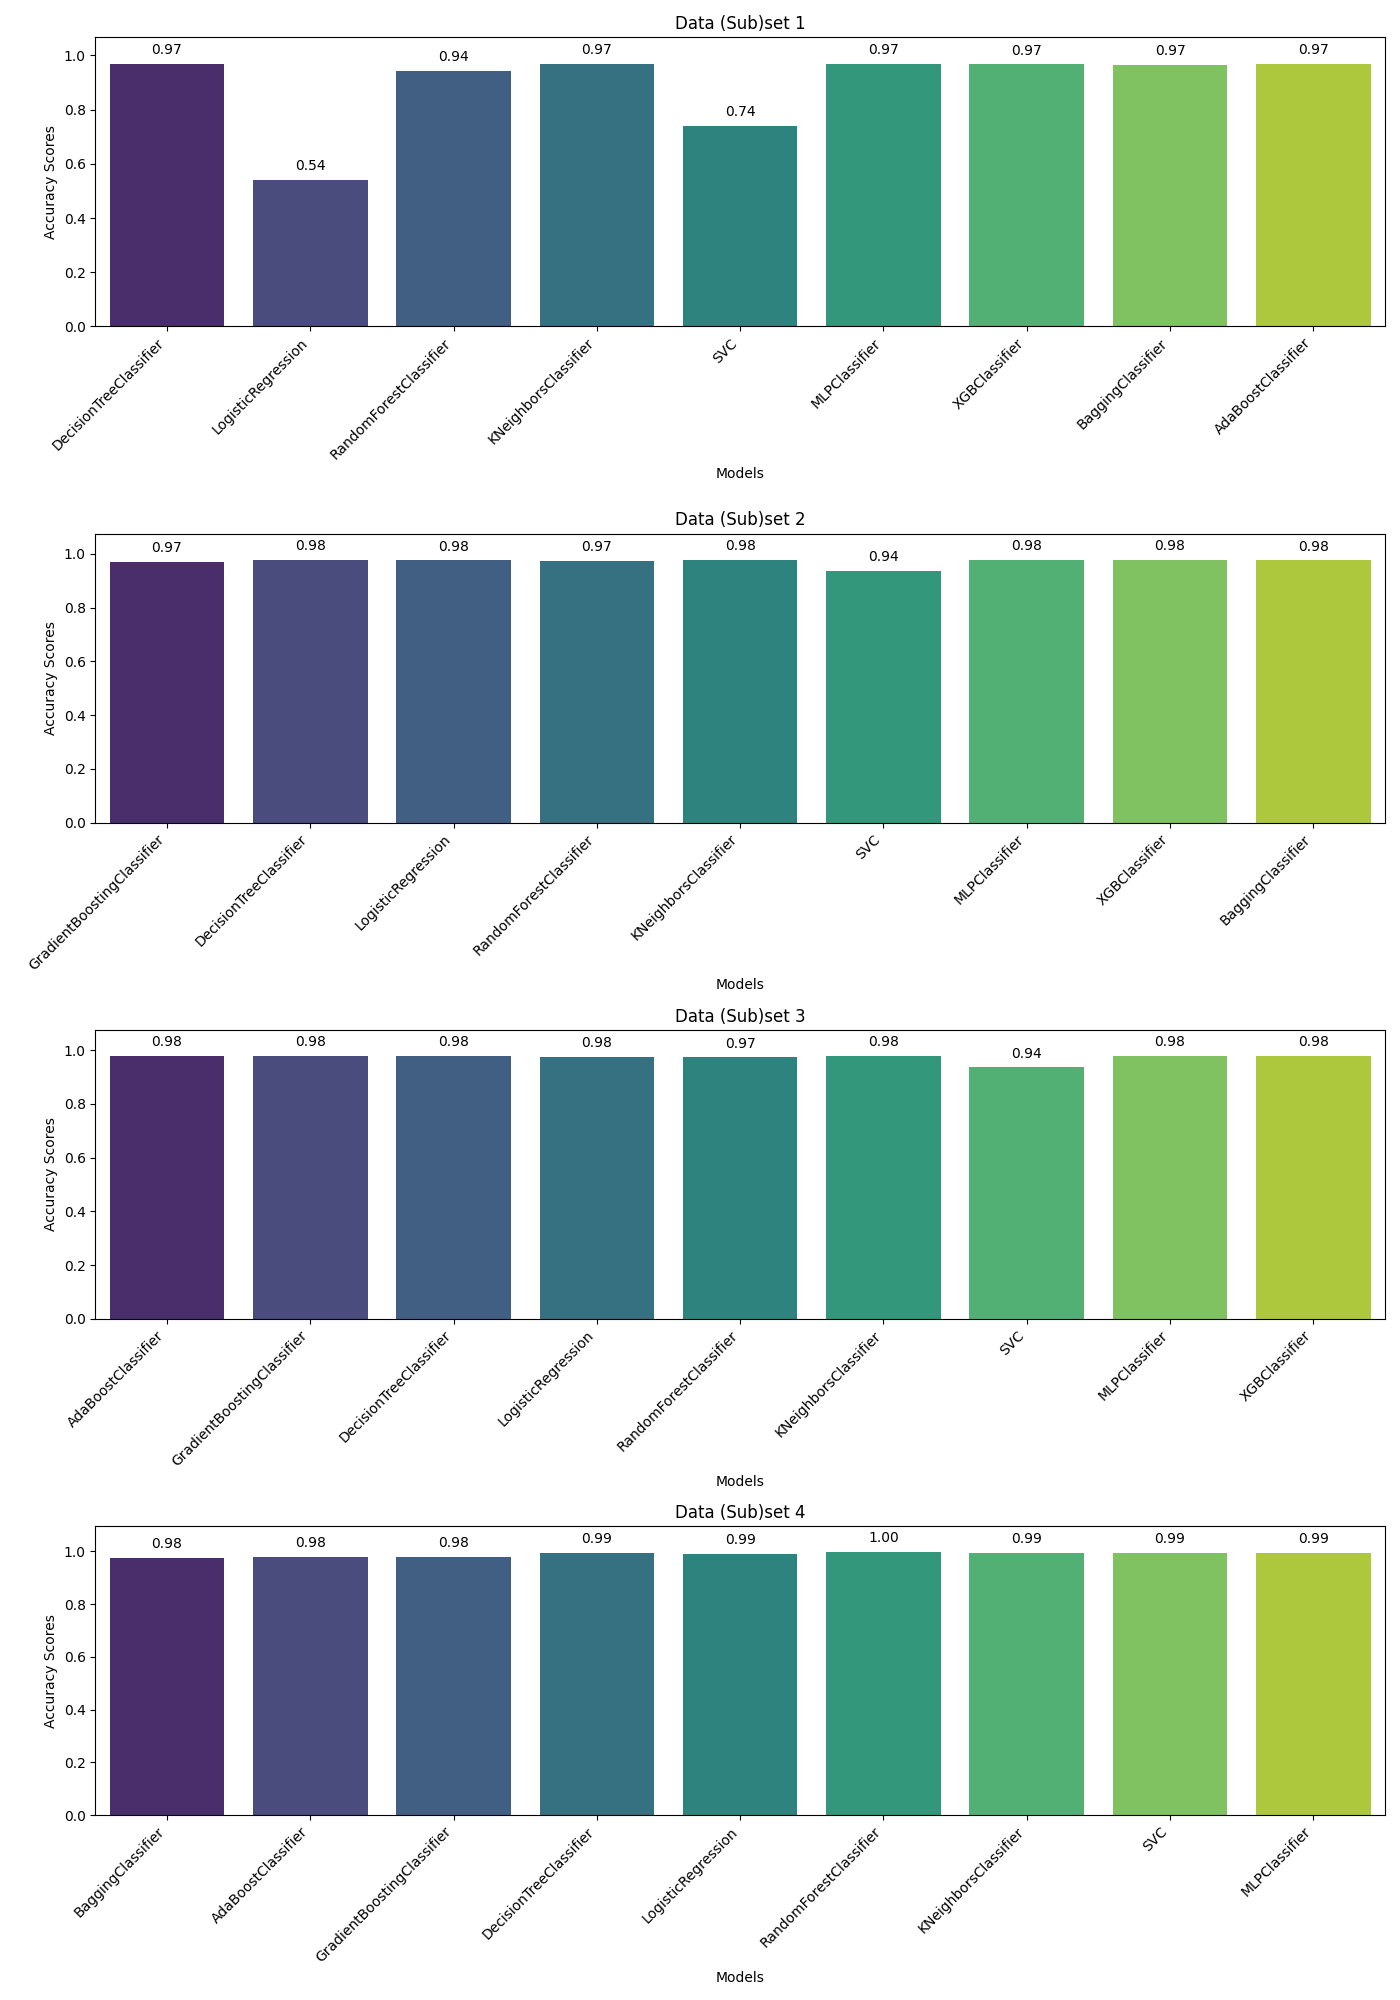
\includegraphics[width=0.8\linewidth]{assets/images/best_classifier/50_data_eval.png}
    \caption{Bar chart illustrating the performance differences of different models on different feature sets (50\% of the training data)}
    \label{fig:eval_bar_scores_50}
\end{figure}

\subsection{In-depth Metrics calculations for the best model}\label{s:calculation}

% Mathematical representation of a confusion matrix used for metric calculations
Based on the following heat map,
\[
\begin{bmatrix}
15950 & 47 \\
35 & 13676 \\
\end{bmatrix}
\]
we evaluate the corresponding scores as follows:

% Inline LaTeX code for calculating various evaluation metrics based on the confusion matrix
\begin{align*}
\text{Accuracy} &= \frac{TP + TN}{TP + TN + FP + FN} = \frac{13676 + 15950}{13676 + 15950 + 47 + 35} = \frac{29626}{29708} \approx 0.9972 \\
\text{Precision} &= \frac{TP}{TP + FP} = \frac{13676}{13676 + 47} = \frac{13676}{13723} \approx 0.9966 \\
\text{Recall} &= \frac{TP}{TP + FN} = \frac{13676}{13676 + 35} = \frac{13676}{13711} \approx 0.9975 \\
\text{Specificity} &= \frac{TN}{TN + FP} = \frac{15950}{15950 + 47} = \frac{15950}{15997} \approx 0.9971 \\
\text{F1 Score} &= 2 \cdot \frac{\text{Precision} \cdot \text{Recall}}{\text{Precision} + \text{Recall}} = 2 \cdot \frac{0.9966 \cdot 0.9975}{0.9966 + 0.9975} \approx 0.9970 \\
\text{False Positive Rate (FPR)} &= \frac{FP}{FP + TN} = \frac{47}{47 + 15950} = \frac{47}{15997} \approx 0.0029 \\
\text{False Negative Rate (FNR)} &= \frac{FN}{FN + TP} = \frac{35}{35 + 13676} = \frac{35}{13711} \approx 0.0026 \\
\text{False Discovery Rate (FDR)} &= \frac{FP}{TP + FP} = \frac{47}{13676 + 47} = \frac{47}{13723} \approx 0.0034 \\
\end{align*}
